\item A small disc of mass \( m \) slides down a smooth hill of height \( h \) without initial velocity and gets onto a plank of mass \( M \) lying on the horizontal plane at the base of the hill (Fig. 1.44). Due to friction between the disc and the plank the disc slows down and, beginning with a certain moment, moves in one piece with the plank.
    \begin{center}
        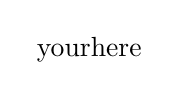
\begin{tikzpicture}
            \node at (0, 0) {{yourhere}};
        \end{tikzpicture}
    \end{center}
    \begin{enumerate}
        \item Find the total work performed by the friction forces in this process.
        \item Can it be stated that the result obtained does not depend on the choice of the reference frame?
    \end{enumerate}\begin{solution}
    \begin{center}
        \begin{tikzpicture}
            \pic at (0, 0) {frame=3cm};
        \end{tikzpicture}
    \end{center}

    \begin{align*}
        \intertext{(a) When the disk slides and comes to the plank, it has a velocity equal to}
        v &= \sqrt{2gb}.\\
        \intertext{Due to friction between the disk and the plank the disk slows down and after some time the disk moves with the plank with velocity \( v' \) (say).}
        \intertext{From the momentum conservation for the system (disk $+$ plank) along horizontal towards right:}
        mv &= (m + M) v' \quad \text{or} \quad v' = \frac{mv}{m + M}\\
        \intertext{Now from the equation of the increment of total mechanical energy of a system:}
        \frac{1}{2}(M + m)v'^2 - \frac{1}{2}mv^2 &= A_{fr}\\
        \intertext{or}
        \frac{1}{2}(M + m) \frac{m^2v^2}{(m + M)^2} - \frac{1}{2}mv^2 &= A_{fr}\\
        \intertext{so,}
        \frac{1}{2} v^2 \left[ \frac{m^2}{M + m} - m \right] &= A_{fr}\\
        \intertext{Hence,}
        A_{fr} &= -\left( \frac{mM}{m + M} \right) gb = -\mu gb\\
        \intertext{(where \( \mu = \frac{mM}{m + M} \) = reduced mass).}
        \intertext{(b) We look at the problem from a frame in which the hill is moving (together with the disk on it) to the right with speed \( u \). Then in this frame the speed of the disk when it just gets onto the plank is, by the law of addition of velocities,}
        v &= u + \sqrt{2gb}.\\
        \intertext{Similarly the common speed of the plank and the disk when they move together is}
        v &= u + \frac{m}{m + M} \sqrt{2gb}\\
        A_{fr} &= \frac{1}{2}(m + M) v^2 - \frac{1}{2}mv^2 - \frac{1}{2}Mu^2\\
        &= \frac{1}{2}(m + M) \left\{ u^2 + \frac{2m}{m + M}u \sqrt{2gb} + \frac{m^2}{(m + M)^2} 2gb \right\}\\
        & \quad - \frac{1}{2}(m + M) u^2 - \frac{1}{2} m2u \sqrt{2gb} - mgh\\
        \intertext{We see that \( A_{fr} \) is independent of \( u \) and is in fact just \( -\mu gb \) as in (a). Thus the result obtained does not depend on the choice of reference frame.}
        \intertext{Do note however that it will be incorrect to apply "conservation of energy" formula in the frame in which the hill is moving. The energy carried by the hill is not negligible in this frame. See also the next problem.}
    \end{align*}
\end{solution}